% !TEX root =  ../Report.tex
\section{Methodology \& Justifications}
\label{sec: Methodology}
This project implements an eight-stage supervised classification pipeline to create directional risk signals for Bitcoin. Daily input data is sourced from three providers: OHLCV price data from Yahoo Finance, on-chain metrics from CoinMetrics, and features engineered using raw OHLCV data and the ta.Lib Python module. The data is processed through sequential stages of Triple Barrier labelling, train/test splitting, feature selection, hyperparameter tuning, and model training for four classifiers: Logistic Regression, SVM-RBF, Random Forest, and XGBoost. Their performance is assessed against both statistical and trading metrics. The pipeline produces three-class outputs (+1 - Oversold, 0 - Neutral, -1 - Overbought) for a 7-day horizon. Intermediate outputs are stored locally as pickle files between stages, allowing each notebook to run independently, with all experiments logged via MLflow for version control. The full architecture is illustrated in Figure \ref{fig:meth Project Pipeline}.

{
  % \setlength{\intextsep}{-5pt}      % space after figure  
  % \setlength{\textfloatsep}{-1pt}   % space before figure
  % \setlength{\floatsep}{-5pt}       % Space between consecutive figures
\begin{figure}[H]
  % \hspace{-0.8cm}
\centering
\begin{minipage}{1\textwidth}
\centering
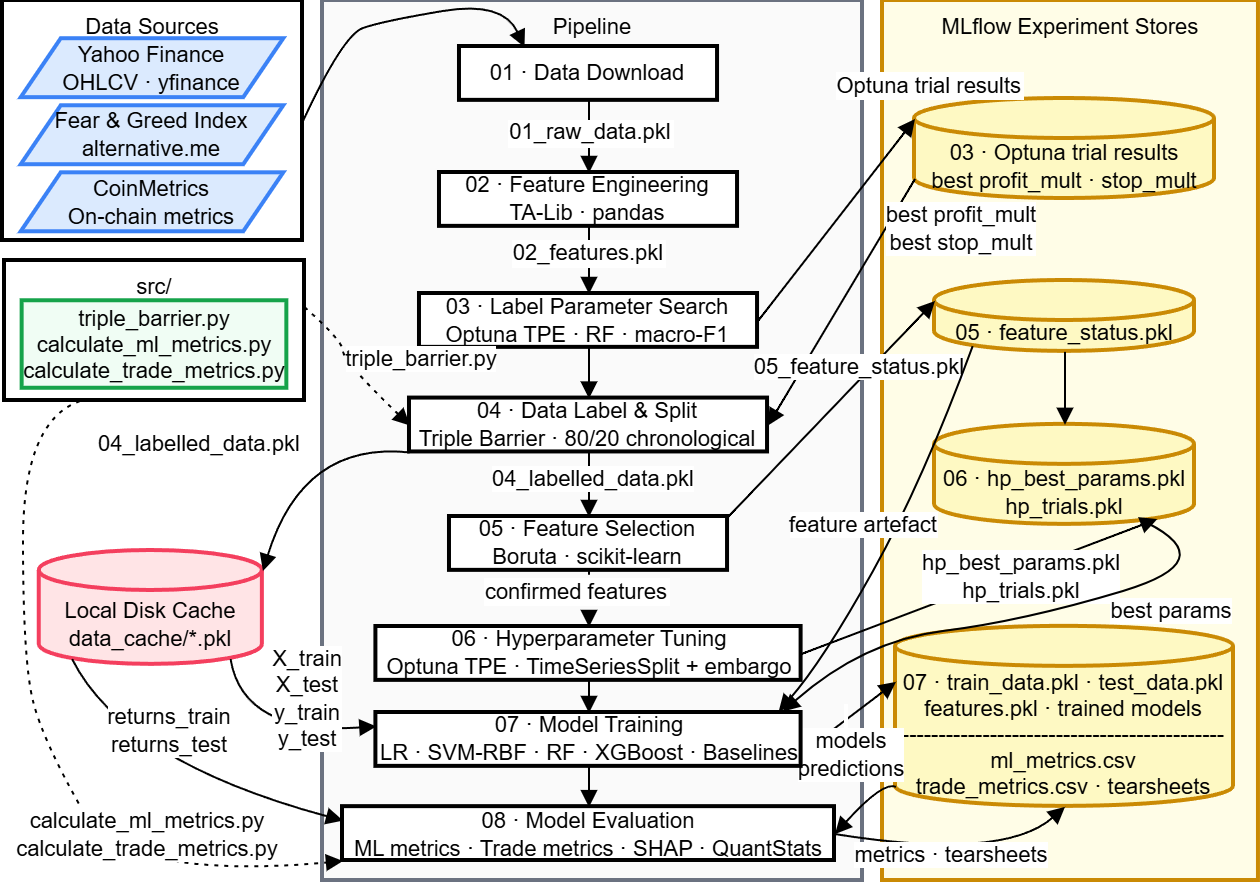
\includegraphics[width=\textwidth]{Report/Chapter3/Flowchart.drawio.png}
\caption{Project Architecture Flowchart showing flow and processing of data.}
\label{fig:meth Project Pipeline}
\end{minipage}
\end{figure}
}
% =============== DATA SOURCES AND ACQUISITION ===============
\subsection{Data Sources \& Acquisition (0.75 pages)}
Three distinct data sources were combined to capture price, sentiment, and on-chain behaviour. One sentence framing why multiple sources are needed - used publicly available sources for accessibility, but needed multiple sources because couldn't find data in one place that wasn't rate limited behind paywalls.
% =============== FEATURE ENGINEERING ===============
\subsection{Feature Engineering (0.5 pages)}
% =============== DATA LABELLING ===============
\subsection{Data Labelling (1.0 pages)}
This is your biggest methodological contribution over prior work — it needs the most space: what it is, the three barriers, EWMA scaling, class imbalance, and the Overbought/Neutral/Oversold mapping
% =============== TRIPLE BARRIER PARAMETERS ===============
\subsection{Optimising Triple Barrier Parmameters (0.75 pages)}
Search space, 100 trials, model-agnostic F1 objective, resulting label distribution — reportable and replicable detail
% =============== TRAIN/TEST SPLIT===============
\subsection{Train/Test Split (0.25 pages)}
\textcolor{red}{Where does discussion of cross validation split in hyperparameter tuning go?}
One paragraph: 80/20 chronological, justify briefly vs the literature convention.
% =============== FEATURE PROCESSING ===============
\subsection{Feature Processing (0.5 pages)}
Mixed RobustScaler/Min-Max strategy, train-only fitting, one table showing which features get which scaler
% =============== FEATURE SELECTION ===============
\subsection{Feature Selection (0.5 pages)}
What Boruta does, why over RFE, your specific parameters, tentative feature handling, final selection decision
% =============== ML MODELS ===============
\subsection{ML Models (0.75 pages)}
One short paragraph per model (LR baseline, SVM-RBF, RF, XGBoost) — what it is and why it suits this problem
% =============== HYPERPARAMETER SELECTION ===============
\subsection{Hyperparameter Tuning (0.5 pages)} 
Optuna TPE, TimeSeriesSplit + embargo, the GT-score objective function, number of trials
\textcolor{red}{Where to say, GT-score model performance downstream was really bad, so switched back to f1 macro?}
% =============== FINAL MODEL TRAINING ===============
\subsection{Final Model Training	(0.1 pages)}
One paragraph only — refit best params on full training set
% =============== EXPERIMENT LOGGING ===============
\subsection{Experiment Logging (MLflow) (0.1 pages)}	
Two to three sentences of justification.
Mlflow has been used throughout the pipeline, used to version control: triple barrier optimised parameters, feature selection, hyperparameter tuning studies and training/evaluation of final models.

\subsection{Model Evaluation	(0.1 pages)}
Forward pointer to Results — metric hierarchy already decided (f1_macro → MCC → trade metrics), just name them here